\chapter{Theory behind SVD}
\label{cha:svd-theory}

Let us begin by giving the formal definition of the SVD factorization,
which is in indeed a theorem (we will restrict ourselves to real
matrices, that is, to matrices whose entries belong to the field
\R{}). \\

\begin{theorem}[Singular Value Decomposition]
\label{thm:SVD}
Let $A$ be a real matrix of $n \times m$ \imply $\exists$ orthogonal matrices
$V$ ($n \times $n) and $U$  ($m \times m$), and diagonal matrix
$\Sigma$ ($m \times n$) \suchthat:

\[
A = U \Sigma \trans{V} 
\]
\\
where $\Sigma$ has the following properties: 
\begin{align*}
 & \Sigma =  diag(\sigma_1,\dots,\sigma_p), & \textds{for} p = min(n,m)  \\
 & \sigma_1 \ge \sigma_2 \ge \dots \ge \sigma_r > 0, & \textds{for} r = rank(A) \\
 & \sigma_{r+1} = \sigma_{r+2} = \dots = \sigma_p = 0 &
\end{align*}
\end{theorem}
\hfill

Note that in the \cref{thm:SVD}, we are considering diagonal
matrices on its more generic form that does not require them to be
square; the definition of diagonal matrix $M$ can simply be that any
element other than $M_{ii}$ becomes zero. \\

Before presenting the proofs, is convenient to provide more context
about the theory behind this matrix factorization (and probably also,
part of the motivation behind). \\

\section{The intuition behind SVD}

In this section we will provide several informal ways of looking at
the SVD factorization, aiming to ignite the formal discussion of next
section (where we prove the SVD theorem). \\

\subsection{SVD as a function composition}

The first thing to remember, is that matrices are the operational
representation of an special type of function between vector
spaces\footnote{The reader is invited to review any Linear Algebra
  textbook, to recall the definition of a vector space}
called linear transformations (also called linear mappings or linear
  functions). We say is an operational representation, in the 
sense that they provide an explicit recipe to apply the
function. Furthermore, the functions they represent are
special, as they have the nice property of preserve algebraic
structure across domain and codomains. Such 
property can be summarized as: \\

\[
f(\alpha x + \beta y) = \alpha f(x) + \beta f(y)
\]
\hfill

Where the addition and products mentioned above, are the vector
addition and multiplication by an scalar; defined for vector
spaces. For the specific case of this work, where we restrict
our attention to real matrices, we can tell that they do represent
functions $f: \R{n} \fromto \R{m}$. \\

In this context of linear functions, the matrix multiplication is the
operational representation of the composition of the associated
functions. A matrix factorization is in essence, a way to understand
what the underlying function does; the whole product can be seen as
serial algorithm, where each matrix represents on particular step or
transformation. Each of the four matrices that appear on the SVD
factorization, has its own function as follows:  

\begin{itemize}
\item $A$ is a function $\func{F_A}: \R{n} \fromto \R{m}$
\item $V$ is a function $\func{F_V}: \R{n} \fromto \R{n}$
\item Same goes for  \trans{V}, which is $\func{F_{\trans{V}}}: \R{n} \fromto \R{n}$
\item $\Sigma$ is a function $\func{F_\Sigma}: \R{n} \fromto \R{m}$
\item $U$ is a function $\func{F_U}: \R{m} \fromto \R{m}$
\end{itemize}
\hfill

Thus, in the context of function compositions, the SVD factorization
can be restated as: \\

\[
\func{F_A}(\vec{x}) = \func{F_U}(\func{F_\Sigma}(\func{F_{\trans{V}}}(\vec{x})))
\]
\hfill

\subsection{SVD as a change of basis}

Next thing to remember, are the specially nice properties of orthogonal
matrices. By definition they are square matrices ($n \times n$), and
their columns form an orthonormal basis of \R{n}; this property
implies that they are invertible, but also, that the inverse is
specially easy to compute: it is just the transpose. In addition,
orthogonal matrices are an special case of change of basis matrices:
if $Q$ is an orthogonal matrix, then it can be seen as a function
which takes vectors in the coordinates of its column basis, and that
spits as result the coordinates in the canonical basis. On the same
line, $\inv{Q}$ does represent the opposite change of basis
(from the canonical coordinates to those in terms of the columns of
$Q$). \\

Having set the proper context, let us restate the SVD factorization as
a sequence of successive transformations:

\begin{enumerate}
\item Start with a vector $\vec{x} \in \R{n}$ in canonical coordinates.
\item Perform a change of basis using matrix \trans{V}, from the
  canonical coordinates to those in terms of the columns of $V$.
\item Once expressed as coordinates of columns of $V$, apply the
  linear transformation $\Sigma$; this not only converts the vector
  from \R{n} to \R{m}, but also expresses the coordinates in terms of
  the columns of $U$.
\item Once transformed, perform another change of basis using matrix
  $U$; from the coordinates of columns of $U$ to the canonical ones
  We end then with a vector in \R{m}.
\end{enumerate}
\hfill

\subsection{SVD as a geometrical interpretation}

And what was the advantage of the factorization then? In simple terms,
decomposing the function behind matrix $A$, as a sequence of three
simpler (easier to understand) transformations. Here the geometric
interpretation helps to complete the picture, as orthogonal (change of
basis) matrices do represent rigid transformation in space, that is,
they do not alter the lengths of vectors (hence, preserve
shapes). Strictly speaking, orthogonal matrices can be decomposed as a
rotation and a reflection; but for geometric intuition, is often
desirable to think in the rotation part only. \\

On the other hand, diagonal matrices are the simplest transformation
possible, they do not change the basis but just expand or contract the
coordinates along the axis given by the basis. Again, if we consider
the generic case of diagonal matrices, a negative element $D_{ii}$
would additional provoke a reflection in the axis $i$; but since the
SVD decomposition produces only positive elements on the diagonal, we
ignore this case and just think in terms of contractions or
expansions along the axes. \\

Armed with this geometrical insight, we can enhance our understanding
of the action of $A$ through the SVD decomposition, by associating to
the simpler operations the corresponding geometrical transformations.
The geometric visualization usually requires a couple of
simplifications: first of all, the dimensions of domain and codomain
must be reduced; as it is easier to visualize things in \R{2} or
\R{3}, than in an arbitrary \R{n}. Given two dimensions fit well in a
screen, let us pick $\R{n} = \R{m} = \R{2}$. \\

Secondly, we need to focus our attention in an specific set of
points (as visualizing the effect of a linear transformation against
``all'' vectors in space, even for \R{2}, is a quite abstract and
complex task). The usual procedure is to pick the vectors in the
unitary sphere in \R{2} (which contains in particular the columns of
$V$, as they are unit orthogonal vectors). \\

Let us proceed now: let the matrix $A$ be of
dimensions $2  \times 2$, the matrices $V$ and $U$ be formed
by unit column vectors $\{\vec{v_1},\vec{v_2}\}$ and $\{\vec{u_1},\vec{u_2}\}$,
respectively; and let matrix $\Sigma$ be $diag(\sigma_1,\sigma_2)$
such that $\sigma_1 > \sigma_2 > 0$. We will additionally assume that
$\sigma_1 > 1$ and $\sigma_2 < 1$, in order to allow them represent an
expansion and contraction, respectively. The previously described steps of
the SVD factorization, can be now augmented with the corresponding
geometrical transformations: \\

\begin{enumerate}
\item Start with unit sphere in \R{2}, with the unit vectors \vec{v_1}
  and \vec{v_2} living inside of it. 
\item Action of \trans{V}: Rotate the space such that \vec{v_1} and
  \vec{v_2} become the new orthogonal basis (this transformation
  leaves the shape of the sphere intact).
\item Action of $\Sigma$: Once rotated, the unit sphere is expanded
  in the direction of \vec{v_1} (per $\sigma_1$), and contracted in the
  direction of \vec{v_2} (per $\sigma_2$). 
\item Action of $U$: Once reshaped, the resulting ellipse is taken
  from the basis $\{u_1,u_2\}$ back to the canonical basis (this
  transformation changes the orientation of the ellipse, given that
  is not a symmetric figure; but still it preserves it shape).
\end{enumerate}
\hfill

These steps can be summarized in the following figure \footnote{Which
  was taken from a \href{http://math.stackexchange.com/questions/243811/visualization-of-singular-value-decomposition-of-a-symmetric-matrix}{MathStackExchange phorum post}, we
  could not locate back the original source though.}: \\

\begin{figure}[h]
  \centering
  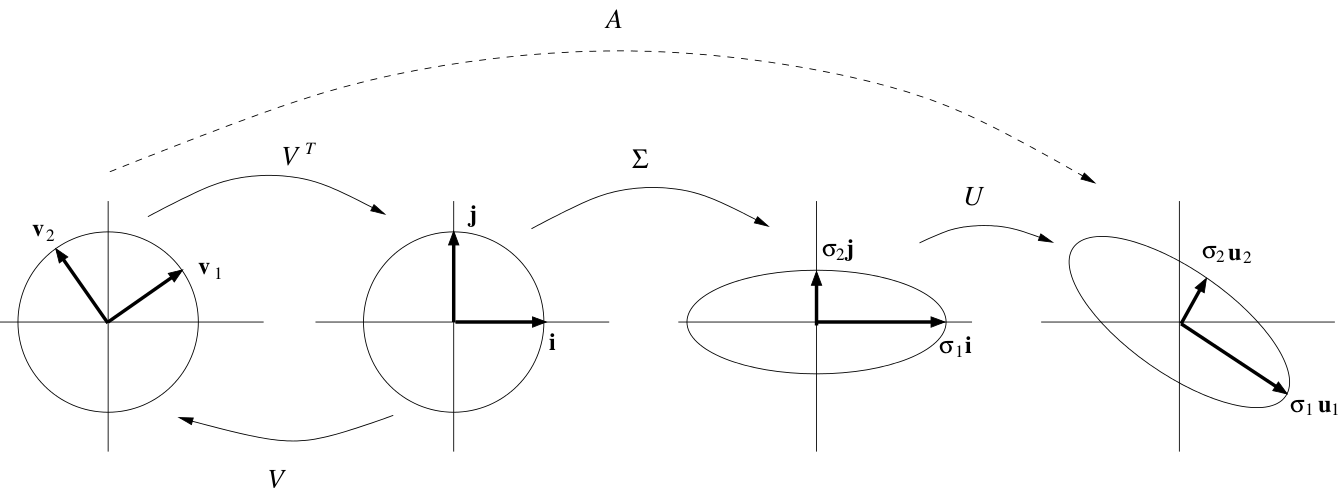
\includegraphics[width=15cm]{svd-geo-diag}
  \caption{Geometrical interpretation of $A = U \Sigma \trans{V}$,
    over the unit sphere.}
  \label{fig:svd-geo-diag}
\end{figure}
\hfill


Although the geometrical interpretation works great for a simple
example in \R{2}, there are a couple of missing details in the action of
matrix $\Sigma$ which are worth mentioning. The first, is that the
dimensions of $\Sigma$ are those of the original matrix ($n \times
m$); therefore, its action is not only expanding or contracting, but
also a migration of space (from \R{n} to \R{m}). If there are more
rows than columns ($m > n$), the transformation $\Sigma$ will produce
a bigger vector than its input (the diagonal entries beyond position
$n$ will be zeroes, which in turn will fill the new vector entries
with zeroes as well; up to $m$ entries). If on the contrary we have
more columns than rows ($m < n$), then the effect will be a truncation
of the input vector (resulting vector has as many entries as rows in
$\Sigma$). In our example, this change of space was not perceived, as $n
= m$. \\

The second omitted detail about the action of $\Sigma$ in 
\cref{fig:svd-geo-diag}, is even more subtle: along with the migration
of space \R{n} to space \R{m}, we are also changing the basis; from
$\{\vec{v_1},\vec{v_2},\dots,\vec{v_n}\}$ to
$\{\vec{u_1},\vec{u_2},\dots,\vec{u_m}\}$. This additional effect may
not be evident at all, but is thanks to an additional property that
is required on the two basis for the SVD factorization to hold:

\[
A\vec{v_i} = \sigma_i\vec{u_i}, \ds{}\forall i=1 \dots r, \ds{}\text{where
} r = rank(A).
\]
\hfill

The above property tells us that the vectors from the two basis were
picked in a very special way: each vector \vec{u_i} is parallel to the
image under $A$ of its associated \vec{v_i}; in other words, the
transformation $A$ maps the \R{n} basis
$\{\vec{v_1},\dots\,\vec{v_n}\}$, into vectors which are parallel to
the \R{m} basis $\{\vec{u_1},\dots\,\vec{u_m}\}$. Given that both basis
are orthonormal, a consequence from this observation is that the
orthogonality of the basis $\{\vec{v_1},\dots\,\vec{v_n}\}$ is preserved
under $A$ (\cite{kalman96}). This is not a trivial property, and not
every basis has it (given $A$ is assumed to be given). This is
actually the key problem of the SVD factorization, and the proofs
provided in the next section, focus around the problem of finding such
special basis.  



\section{The SVD proofs}
The rest of this chapter provides more theoretical background about
the SVD decomposition, in particular, it provides two different proofs of
\cref{thm:SVD}:

\begin{itemize}
  \item Algebraic proof using the Spectral Theorem.
  \item Geometric proof (implicitly using Compactness).
\end{itemize}
\hfill

Each one of those proofs is intended to bring a
different perspective, about such an important result as SVD is. The
list is not exhaustive of course, there could be many more ways of 
proving it; but hopefully the short list presented here, will give the
reader an idea about the rich theory behind this decomposition. \\

As with any mathematical theorem, proving is done based on previous
results; since this is not a text book, we can not afford the luxury
of proving every auxiliary theorem we use. However, we made an effort
for at least mentioning explicitly the theorems; pointing to
references, when possible, about their respective proofs. For some few
cases (like the Spectral Theorem), we did include the proof of the
auxiliary theorem as well.

\subsection{Algebraic proof (using Spectral Theorem)}

The proof in this section relies on the Spectral Theorem, which says
that we can diagnonalize a symmetric matrix. Instead of jumping right
away to the proof of SVD with such heavy machinery, we prefer a
gradual approach consisting of the following steps: \\

\begin{itemize}
\item Emphasize that the main task of SVD factorization, is to find a
  basis for \R{n} whose orthogonality is preserved under $A$.
\item Introduce Fundamental Theorem of Linear Algebra along the four
  subspaces related to an arbitrary matrix 
  $A$.
\item Motivated by the discussion about the four subspaces, bring to the
  picture the symmetric matrix $\trans{A}A$ (aka the gramian), and
  state the properties we will need for the SVD proof.
\item The symmetric nature of $\trans{A} A$, will justify the
  usage of the Spectral Theorem; which we proceed to prove.
\item Finally, we  prove SVD \cref{thm:SVD} itself using the Spectral
  Theorem as the main tool, but we also use  the auxiliary theorems
  stated along the way.
\end{itemize}
\hfill

\subsubsection{The factorization properties}

Let us resume the discussion from last section, where we claim that
all we needed  was that the vectors of
the two bases had the property of $A\vec{v_i} =
\sigma_i\vec{u_i}$. Let us prove such claim, and show that if that
condition is met, then SVD factorization can be achieved. \\

\begin{theorem}[SVD Part 1: the factorization]
\label{thm:SVD1}
Let $A$ be a real matrix of $n \times m$,\text{if } $\exists$
orthonormal basis $\{\vec{v_1},\vec{v_2},\dots,\vec{v_n}\}$ for \R{n},
and another orthonormal $\{\vec{u_1},\vec{u_2},\dots,\vec{u_m}\}$ for
\R{m} which hold the following property:

\[
A\vec{v_i} = \sigma_i\vec{u_i}, \ds{}\forall i=1 \dots r, \ds{}\text{where
} r = rank(A).
\]
\\
Then we can factorize matrix $A$ as $U \Sigma \trans{V}$. \\

where 

\begin{itemize}
\item $V$ is the orthogonal matrix formed by arranging vectors
\vec{v}\apos{s}
\item matrix $U$ is defined similarly for vectors
\vec{u}\apos{s}
\item The only non zero entries of diagonal matrix $\Sigma$, are 
those $\Sigma_{ii} = \sigma_i > 0$ for $1 <= i <= r$.
\end{itemize}
\end{theorem}
\hfill

\begin{proof}
This \cref{thm:SVD1} is mentioned in \cite{kalman96}, though not
explicitly proved. Let us do it here, following the advice from
\cite{strang88}, that the trick is to think about a matrix
multiplication $A B$, as the result of matrix-vector products ($A
\vec{b_i}$), where the vectors are the columns of $B$. In our particular
case, the matrix-vector products we have are $A\vec{v_i}$; if we
arrange them as columns of a new matrix it would be equal to $A
V$. That is: 

\[
\begin{bmatrix}
  A\vec{v_1} \mid A\vec{v_2} \mid \cdots \mid A\vec{v_n} 
\end{bmatrix} = 
A 
\begin{bmatrix}
  \vec{v_1} \mid \vec{v_2} \mid \cdots \mid \vec{v_n} 
\end{bmatrix} =
AV
\]
\hfill

Since we do not have product $AV$ in our target result, let us use the
fact that $V$ is orthogonal; which in particular implies that \inv{V}
= \trans{V}. That allows to focus on an target result, which involves
$AV$: 

\[
A   = U \Sigma \trans{V} \ds{\iff}
A V = U \Sigma V \trans{V} \ds{\iff}
A V = U \Sigma
\]
\hfill

So we can focus in proving that $A V = U \Sigma$. Let us work
the left side first, which per our previous observation that
$A\vec{v_i}$ are the columns of matrix product $AV$, and per hypothesis
that $A\vec{v_i} = \sigma_i\vec{u_i}$ can be rewritten as follows:

\begin{align*}
  & A V &= \\
  & A \begin{bmatrix}
    \vec{v_1} \mid \vec{v_2} \mid \cdots \mid \vec{v_n} 
  \end{bmatrix} &= \\
  & \begin{bmatrix}
      A\vec{v_1} \mid A\vec{v_2} \mid \cdots \mid A\vec{v_n} 
    \end{bmatrix} &= \\
  & \begin{bmatrix} 
      \sigma_1\vec{u_1} \mid \sigma_2\vec{u_2} \mid \dots \mid \sigma_r\vec{u_r} 
      \mid A\vec{v_{r+1}} \mid A\vec{v_{r+2}} \mid \dots \mid A\vec{v_{n}} 
    \end{bmatrix}
\end{align*}
\hfill

Let us now develop the left side $U \Sigma$ by thinking again in the
result, as formed by columns of the form $U \vec{\Sigma_i}$ (where
  \vec{\Sigma_i} is the $i$th column of diagonal matrix $\Sigma$): 

\begin{align*}
  & U \Sigma &= \\
  & \begin{bmatrix}
      U\vec{\Sigma_1} \mid U\vec{\Sigma_2} \mid \cdots \mid U\vec{\Sigma_n} 
    \end{bmatrix} &= \\
  & \begin{bmatrix}
      U\vec{\Sigma_1} \mid U\vec{\Sigma_2} \mid \cdots \mid U\vec{\Sigma_r} \mid
      U\vec{\Sigma_{r+1}} \mid U\vec{\Sigma_{r+2}} \mid \cdots \mid U\vec{\Sigma_{n}} 
    \end{bmatrix} &= \\[1ex]
  & \begin{bmatrix}
      U\vec{\Sigma_1} \mid U\vec{\Sigma_2} \mid \cdots \mid U\vec{\Sigma_r} \mid
      \smash{\underbrace{U\vec{0} \mid U\vec{0} \mid \cdots
          \mid U\vec{0}}_{n - r}}
    \end{bmatrix} &= \\[2.5ex]
  & \begin{bmatrix}
      U\vec{\Sigma_1} \mid U\vec{\Sigma_2} \mid \cdots \mid U\vec{\Sigma_r} \mid
      \smash{\underbrace{\vec{0} \mid \vec{0} \mid \cdots \mid \vec{0}}_{n-r}} 
    \end{bmatrix} &= \\[0.5ex]
\end{align*}

The last $n - r$ zero vectors were a consequence of the definition of
$\Sigma$, which only has non-zeroes on diagonal up to position
$r$. And the columns $U\vec{\Sigma_i}$ can be simplified further, as
each column vector \vec{\Sigma_i} has the only non-zero entry
$\sigma_i$ precisely at position $i$. Hence, only column $i$ of $U$
survives after multiplying it by \vec{\Sigma_i}, and the final effect
is just the multiplication by scalar $\sigma_i$:

\[
 U \Sigma = 
\begin{bmatrix}
   U\vec{\Sigma_1} \mid U\vec{\Sigma_2} \mid \cdots \mid U\vec{\Sigma_r} \mid
   \smash{\underbrace{\vec{0} \mid \vec{0} \mid \cdots \mid \vec{0}}_{n-r}}
\end{bmatrix} = 
\begin{bmatrix}
   \sigma_1\vec{u_1} \mid \sigma_2\vec{u_2} \mid \cdots \mid \sigma_1\vec{u_r} \mid
   \smash{\underbrace{\vec{0} \mid \vec{0} \mid \cdots \mid \vec{0}}_{n-r}}
\end{bmatrix}
\]
\hfill

If we put together the developments for each side, we are almost done:

\begin{align*}
  & A V &= \\[1.5ex]
  & \begin{bmatrix}
    \sigma_1\vec{u_1} \mid \sigma_2\vec{u_2} \mid \cdots \mid \sigma_r\vec{u_r} \mid
    \smash{\underbrace{A\vec{v_{r+1}} \mid A\vec{v_{r+2}} \mid \cdots \mid A\vec{v_{n}}}_{n-r}}
  \end{bmatrix}  &= \\[3.5ex]
  & \begin{bmatrix}
    \sigma_1\vec{u_1} \mid \sigma_2\vec{u_2} \mid \cdots \mid \sigma_1\vec{u_r} \mid
    \smash{\underbrace{\vec{0} \mid \vec{0} \mid \cdots \mid \vec{0}}_{n-r}}
  \end{bmatrix} &= \\[1.5ex]
  & U \Sigma
\end{align*}
\hfill

\end{proof}

It can be observed that the proof is not complete, though we are
almost done; in order to achieve an equality between $AV$ and
$U\Sigma$, the only missing part is that the last $n-r$ items on each
side are the same. This can be restated in an additional theorem: \\

\begin{restatable}[SVD Part2: basis of null space]{theorem}{svdtwo}
\label{thm:SVD2}
Assuming same definitions as \cref{thm:SVD1}, it must be the case that:

\[
A\vec{v_i} = \vec{0}, \textds{for} (r+1) \le i \le n
\]

which is equivalent to say that those vectors \vec{v_i}, belong to the
null space of $A$ (they actually form a basis of it).
\end{restatable}

We do not have yet the required machinery to proof 
\cref{thm:SVD2}, but we will do it on the next section, when we
introduce the subspaces associated with each matrix $A$. \\

\subsubsection{The Fundamental Theorem of Linear Algebra}

In order to proof the pending \cref{thm:SVD2} from previous
section, we need to present the four subspaces that an arbitrary
matrix $A$ introduces. But before that, a few important
definitions and remarks: \\

\begin{itemize}
    \item Matrix application $A\vec{x}$ can be seen as a linear
      combination of the columns of $A$:
      \[
      A\vec{x} = 
      \begin{bmatrix}
        \vec{A_1} \mid \vec{A_2} \mid \cdots \mid \vec{A_n}
      \end{bmatrix} \vec{x} = 
      \sum_{i=1}^n x_i \vec{A_i}
      \]
  \item Subspace: A subset of a vector space, which is itself a
    vector space (that is, contains the \vec{0} and is closed under
    the addition and multiplication by an scalar). 
  \item Dimension: Is the size of any basis of a vector space (an
    important result in Linear Algebra, shows that all the basis must
    have the same number of elements; hence, the dimension is a property of the
    space itself). The dimension of a vector space (or subspace) $V$
    is denoted as $\dim{V}$.
  \item Given vector space $V$ and a subspace $W \subset V$ , the
    subspace $\ortc{W} \subset V$ consists of all
    the vectors of $V$ which are orthogonal to all the vectors of
    $W$. $\ortc{W}$ is called the orthogonal complement of $W$.
\end{itemize}
\hfill

Now is right time to talk about the subspaces: we already established
that each matrix of $m \times n$, can be seen as the operational
representation of a linear transformation with signature $\R{n}
\fromto \R{m}$. The action of $A$, in transforming the vectors from
one space to the other, has an interesting effect on each side: both
domain (\R{n}) and codomain (\R{m}), are broken in two orthogonal
pieces. Those pieces actually, happen to be subspaces and their basis
are contained on the matrices $V$ and $U$ of the SVD factorization! But
let us explain piece by piece; a good start, is the column space. \\

The column space of a matrix $A$, is pretty much the concept of the
image of a function; that is, the set of all vectors in 
$A\vec{x} \in \R{m} \suchthat \vec{x} \in \R{n}$, and it is denoted as
$\C{A}$. Another way of looking at it (per one of the remarks above),
is that each application 
of the linear transformation $A$ (that is, each $A\vec{x}$), converts
the input vector \vec{x} into a linear combination of the columns of
A; therefore, $\C{A}$ is the spanning set generated by the
columns of $A$. It can be proved that this subset is actually a
subspace of \R{m}. \\

The next subspace is also clearly understood, is the so called
null space of $A$. It consists of all the solutions to the homogeneous
system $A\vec{x} = \vec{0}$ and is denoted as $\N{A}$. In the
language of transformations, is the set 
of all vectors $\vec{x} \in \R{n}$ that function $A$ compresses into the zero
vector of \R{m}. This subset at least contains the vector \vec{0}, but
in general it will contain much more vectors (only the non-singular
matrices have $\N{A} = \{\vec{0}\}$). Again, it can be proved
that this subset is also a subspace (though this one belongs to \R{n}). \\

The next two subspaces, are not that intuitive to introduce; unless we
think now in terms of the transformation represented by matrix
\trans{A}. This matrix represents a linear transformation that goes
into the opposite direction of $A$, that is, from \R{m} to \R{n}. If
we think in the image of this function $\{\trans{A}\vec{y} \in \R{n} \mid
y \in \R{m} \}$, an interesting realization comes to the picture: what if we
apply the same idea as before, that $\trans{A}\vec{y}$ is a linear
combination of the columns of $\trans{A}$: \\

\[
\trans{A}\vec{y} = 
\begin{bmatrix}
  \vec{(\trans{A})_1} \mid \vec{(\trans{A})_2} \mid \cdots \mid \vec{(\trans{A})_m}
\end{bmatrix} \vec{y} = 
\sum_{i=1}^m y_i \vec{(\trans{A})_i} = 
\sum_{i=1}^m y_i (\text{row $i$ of $A$})
\]
\hfill

In order words, columns of \trans{A} are the rows of $A$, therefore;
the column space of \trans{A} is precisely the row space of original
matrix $A$; this is denoted as \C{\trans{A}} and it can also
be proved that it is a subspace of \R{m}. The last and fourth
subspace, comes from considering the null space of \trans{A}; that is,
those vectors \vec{y} in \R{m} which are compressed into the zero
vector of \R{n}. Is not hard to prove that this is a subspace as
well; it is called the left null space of $A$, and denoted as
\N{\trans{A}}. \\

Summarizing, the four subspaces associated to any
matrix $A$ of $m \times n$ are the following (intuitive proofs that
all of them are indeed subspaces can be found in \cite{strang88}): \\

\begin{itemize}
\item \C{\trans{A}}: row space, lives in \R{n}
\item \N{A}: null space, lives in \R{n}
\item \C{A}: column space, lives in \R{m}
\item \N{\trans{A}}: left null space, lives in \R{m}
\end{itemize}
\hfill

The first thing we note is the intentional grouping of these subspaces;
while \C{\trans{A}} and \N{A} belong to \R{n} [the domain of $A$],
\C{A} and \N{\trans{A}} belong to \R{m} [the codomain of $A$]. These
pairs of subspaces have more in common than merely sharing same
hosting space, they are orthogonal with each other! This is the time
to meet what Strang calls the Fundamental Theorem of Linear Algebra
(part II\footnote{Strang presents the theorem parts in the opposite order
  in \cite{strang88};
  but we preferred to keep our own order, aiming to match better the
  flow of deductions presented in this work.}): \\

\begin{theorem}[Fundamental Theorem of Linear Algebra (part II)]
\label{thm:Fund1}
Let $A$ be a real matrix of $n \times m$, then 

\[
\C{\trans{A}} = \ortc{\N{A}} \ds{\land} \C{A} = \ortc{\N{\trans{A}}}
\]
\end{theorem}
\hfill

\begin{proof}
Let $\vec{x} \in \N{A}$, then \vec{x} satisfies the equation $A\vec{x}
= \vec{0}$; but the resulting vector in \R{m} has as entries the dot product
of \vec{x} with the rows $r_i$ of $A$, therefore, the equation $A\vec{x} =
\vec{0}$ can be rewritten as $m$ equations of the form:

\[
r_i \cdot \vec{x} = 0, \ds{for } 1 \le i \le m
\]

which is essentially saying that the vector \vec{x} is orthogonal to
all the rows $r_i$ of $A$; therefore, it is orthogonal to every linear
combination of them. But those linear combinations are precisely the
row space \C{\trans{A}}; thus $\C{\trans{A}} \perp \N{A}$, or,
reusing previously introduced terminology (see remarks section), we
can say that the row space is the orthogonal complement of the null
space (which is written as $\C{\trans{A}} = \ortc{\N{A}}$).  \\ 

An analogous argument can be constructed for \C{A} and \N{\trans{A}},
using the equation $\trans{A}\vec{y} = \vec{0}$ (details are in
\cite{strang88}). Thus, we can also conclude that the column space is
the orthogonal complement of the left null space (which can be written as $\C{A} =
\ortc{\N{\trans{A}}}$). 
\end{proof}

Having established the orthogonality of these subspaces, allow us to
introduce a secret weapon that will finally help us prove the pending
\cref{thm:SVD2}. This weapon is another theorem that establishes a
relationship between the dimension of any subspace and its orthogonal
complement \footnote{The
  name was provided by us, as Lang does not name it in his book
  \cite{lang04}.}: \\

\begin{theorem}[Orthogonal Complement Dimension Theorem]
\label{thm:ortdim}
Let $W$ any subspace of \R{n}, then is the case that

\[
\dim{W} + \dim{\ortc{W}} = n
\]
\end{theorem}
\hfill

An even more generic version of this theorem is proved by Lang in
\cite{lang04} (theorem 2.3 in that book), and it basically says that
if we take any subspace and its orthogonal complement together, they
form the entirety of the host space! Another way of seeing this
result, is saying that the host space $V$ is the direct sum of the
subspace $W$ and its orthogonal  complement (denoted as $V = W \oplus
\ortc{W}$). Intuitively, the notion 
of a direct sum tells us that there is nothing out of the union of the
subspace $W$ and its orthogonal complement \ortc{W}; every vector in
the original space can be expressed as a sum $x_1 + x_2$ (where
each $\vec{x_1} \in W$ and $\vec{x_2} \in \ortc{W}$, and $W$), and
\ortc{W} do not share anything other than zero vector ($W \cap
\ortc{W} = \{\vec{0}\}$). \\

Using this weapon, we can finally prove the pending 
\cref{thm:SVD2}, which was about proving that the last $n-r$ vectors
of $V$ actually belong to \N{A}. \\

\svdtwo*

\begin{proof}
By hypothesis we know that 

\[
A\vec{v_i} = \sigma_i\vec{u_i}, \ds{}\forall i=1 \dots r, \ds{}\text{where
} r = rank(A).
\]
\\

Since the vectors \vec{u_i}\apos{s} form a basis of \R{m}, that
implies none of them can be zero; therefore $A\vec{v_i} \ne \vec{0}
\ds{}\forall i=1 \dots r$. By definition, such condition implies that
those vectors $v_i \notin \N{A}$, but since $\R{n} = \C{\trans{A}} \oplus \N{A}$,
then the only other option for those vectors
$\{\vec{v_1},\vec{v_2},\dots,\vec{v_r}\}$ is to belong to the row
space \C{\trans{A}}. Actually, since they are all orthogonal, they form
a basis of \C{\trans{A}} (because $\dim{\C{\trans{A}}} = \func{rank}(A) =
r$). Let us call this basis $B_r$. \\

Let $\vec{v_i} \in \R{n}$, which also belongs to
$\{\vec{v_{r+1}},\vec{v_{r+2}},\dots,\vec{v_n}\}$; since \vec{v_i}
is orthogonal to every vector in $B_r$ (as all the \vec{v}\apos{s}
form an orthonormal basis of \R{n}), then \vec{v_i} can not belong
to the subspace generated by $B_r$, which happens to be
\C{\trans{A}}. Using again the fact that $\R{n} = \C{\trans{A}} \oplus
\N{A}$, we can tell that the only other option for $\vec{v_i}$ is to
belong to the nullspace \N{A}. And by definition of nullspace:

\[
A\vec{v_i} = \vec{0}, \ds{}\forall i=(r+1) \dots n
\]
\hfill

which completes the proof. Mirroring the reasoning about basis $B_r$
of the row space, we can also tell that the vectors
$\{\vec{v_{r+1}},\vec{v_{r+2}},\dots,\vec{v_n}\}$ form a basis of the
null space \N{A}. 
\end{proof}

Since we established already the orthogonality between the four
subspaces of matrix $A$, we can simply apply \cref{thm:ortdim}
to them in pairs (depending on whether they are hosted on same space),
and derive the following equations: \\

\begin{enumerate}
\item In \R{n}: $\C{\trans{A}} = \ortc{\N{A}} \implies
  \dim{\N{A}} + \dim{\C{\trans{A}}} = n$
\item In \R{m}: $\C{A} = \ortc{\N{\trans{A}}} \implies 
  \dim{\N{\trans{A}}} + \dim{\C{A}} = m$
\end{enumerate}
\hfill

These two equations are what Strang calls the Fundamental Theorem of
Linear Algebra (Part I); further references are \cite{strang88} and
\cite{strang93}. The two parts of such theorem together, basically
describe what are the subspaces generated by matrix $A$, what is the
relationship among them (orthogonality) and what are their
dimensions. The \cref{fig:fund} below (taken from
\cite{strang88}), summarizes both parts of this important theorem:
\\

\begin{figure}[h]
  \centering
  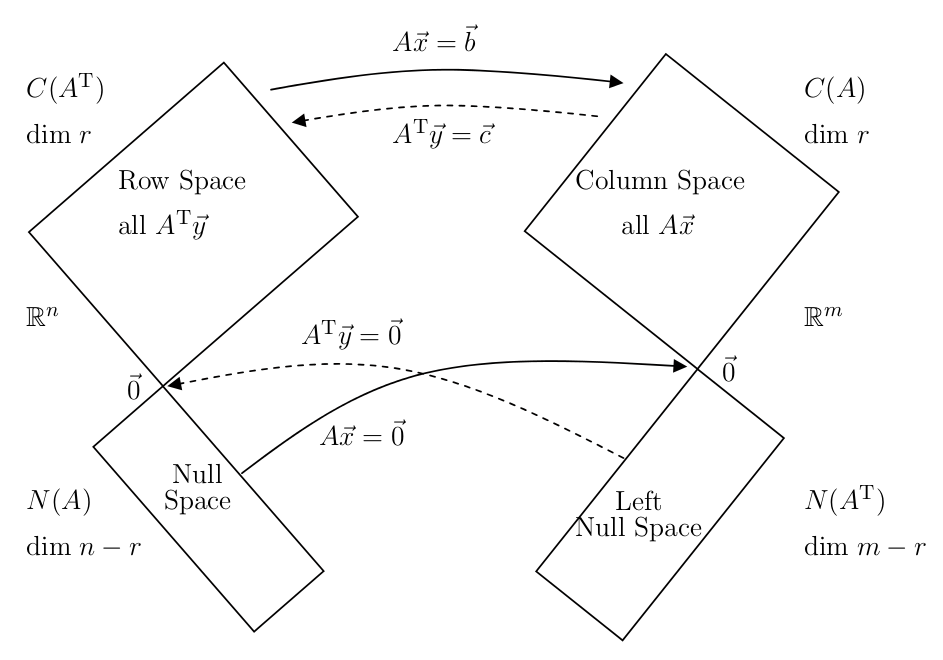
\includegraphics[width=14cm]{fund}
  \caption{Visualization of the Fundamental Theorem of Linear Algebra}
  \label{fig:fund}
\end{figure}
\hfill

Strang goes further in contextualizing the SVD factorization in the
above diagram (\cite{strang93}), by noting that the columns of the
matrices $V$ and $U$, actually contain the basis of these four
subspaces: 

\begin{itemize}
\item The orthogonal matrix $V$ contains a basis for the row space
  \C{\trans{A}} in the first $r$ columns, and a basis for the null
  space \N{A} in the last $n-r$ columns. We showed this already while
  proving \cref{thm:SVD2}. 
\item The orthogonal matrix $U$ contains a basis for the column space
  \C{A} in the first $r$ columns, and a basis for the left null
  space \N{\trans{A}} in the last $m-r$ columns. 
\end{itemize}
\hfill

The last observation makes the SVD factorization even more astonishing
and intriguing: not only it allows one to understand the true nature of
an arbitrary matrix $A$, by explicitly giving the two change of basis
that make $A$ a positive diagonal matrix $\Sigma$ (having just
compressions and expansions). Also, if we consider a basis as a 
representation of a vector space; then the matrices $V$ and $U$ of the
SVD factorization can be 
considered a representation of the four subspaces generated by that
particular matrix $A$. Putting together the three matrices as in $A =
U\Sigma\trans{V}$, gives the truly complete picture about the effects
of transformation $A$. 


\subsubsection{The gramian matrix $\trans{A}A$}

We brought the \cref{fig:fund} not only to illustrate the
Fundamental Theorem of Linear Algebra, but also to justify the
introduction of the matrix $\trans{A}A$ (also called the gramian
matrix of $A$). From the figure, it can be seen that the matrix $A$
takes the row space \C{\trans{A}} into the column space \C{A}; and we
know that both subspaces have the same dimension $r =
\func{rank}(A)$. As Strang explains in \cite{strang88}, the
dimensions of the domain \R{n} and codomain \R{m} do not tell the real
story about the linear transformation behind $A$; it is rather the
dimensions of \C{\trans{A}} and \C{A}. \\

If we just pay attention to
those subspaces, then the matrix $A$ behaves like a bijection (this is
proved in \cite{strang88}); that is, if we took the submatrix of
dimensions $r \times r$ that results from eliminating dependent rows
and columns in $A$, such matrix would be invertible and the inverse would
take the column space \C{A} into the row space \C{\trans{A}}. 
Thus, the real information of matrix $A$ lies in the one-to-one
transformation of \C{\trans{A}} into \C{A}; the null spaces in both
sides (\N{A} and \N{\trans{A}}) do not contribute much to the
the transformation $A$, as they just get compressed to the zero vector. \\

Alright, putting aside the null spaces and focusing only in the
bijection that $A$ performs between the row and column spaces, one may
be tempted to think from \cref{fig:fund} that the transpose of $A$
(denoted as \trans{A}), is actually the inverse of $A$ in the context
of those subspaces. But as Strang promptly clarifies in
\cite{strang88}, that honor belongs only to the actual inverse of
A. We refer to the inverse here, not in the regular sense, but
restricted to the subspaces \C{\trans{A}} and \C{A} (that is, we are
talking about the inverse of the submatrix of $k \times k$ that we
mentioned above). The effect of \trans{A} is 
correct at the level of the whole subspace \C{A}; it takes it back to
\C{\trans{A}}. But the vectors that were originally mapped by $A$, are
not necessarily recovered after applying \trans{A} to that image
$A\vec{x}$. \\

One particular way of reinforcing the fact that \trans{A} is not the
inverse, is by an indirect measure. If we take the dot product between
the starting point \vec{x} in \R{n}, and the result of applying
\trans{A} to its image $A\vec{x}$, that would give us an indication of
how close or distant they are (in the end, the dot product and the
orthogonal projection are intimately related). If the starting and
final vectors happen to be the same, the cited dot product shall be
$\norm{x}_2^2$ (where $\norm{.}_2$ represents the known euclidean
distance). Let us confirm ourselves that is not the case: \\

\begin{align*}
& \vec{x} \cdot (\trans{A} A\vec{x}) &= \\
& \trans{\vec{x}} (\trans{A} A\vec{x}) &= \\
& (\trans{\vec{x}} \trans{A}) (A\vec{x}) &= \\
& \trans{(A\vec{x})} (A\vec{x}) &= \\
& (A\vec{x}) \cdot (A\vec{x}) &= \\
  & \norm{A\vec{x}}_2^2 &\le 
& \norm{A}_2^2 \norm{\vec{x}}_2^2
\end{align*}
\hfill

From the above development, we can see indeed that $\vec{x}
\cdot (\trans{A} A\vec{x}) \ne \norm{x}_2^2$; actually, in the last step
we used a general property of matrix norms, which in particular applies
to the extension of the vector norm $\norm{.}_2$ to matrices. We will not
define it formally, but it suffices to keep the intuition that norm of
$A$, denoted as $\norm{A}_2$, is a measure of the distortion that the linear
transformation $A$ does on the space (is actually the maximum
distortion on the unit sphere). In the last step we can see that 
such measure of distortion, is precisely one of the factors that
prevents that simply taking the transpose \trans{A} as a way back,
sends us to the starting point in the row space. \\

Above reasoning is a further argument for $\trans{A} \ne \inv{A}$;
such special property only applies to orthogonal matrices (like the
$U$ and $V$, which appear in the SVD factorization). For orthogonal
matrices, $\trans{A} A = I$, where $I$ is the identity matrix; and
though that does not occur in general for an arbitrary matrix $A$, the
function composition represented by $\trans{A}A$ is quite interesting;
it may not be the identity function, but at least it has one of its
properties: \\

\[
\trans{(\trans{A}A)} = \trans{A}\trans{(\trans{A})} = \trans{A}A
\]
\hfill

The matrix $\trans{A}A$ (called gramian) is equal to its transpose, which is the
definition of a symmetric matrix. This particular symmetric matrix
is quite important for us, as it represents the bridge between the SVD
factorization and the Spectral Theorem; in short, the Spectral Theorem
guarantees that any symmetric matrix is diagonalizable, and applying such
factorization to our special matrix $\trans{A}A$, give us the two bases
that we need to build the SVD factorization (which happen contain, the
bases of the four subspaces of $A$). These details will be developed in
the next two sections. For the moment, we will just finish the current one
by establishing a few more facts about $\trans{A}A$, which
show its close connection with $A$. \\

Is not hard to show that $\trans{A}A$ and $A$ share the same null
space; and that actually implies that the rank of both matrices is
the same. Let us state that in a theorem and prove it:

\begin{theorem}[Rank of the Gramian Matrix]
\label{thm:gramr}
Let $A$ be a real matrix of rank $r$ $\implies$ its gramian matrix
$\trans{A}A$ has the same rank $r$.
\end{theorem}
\hfill

\begin{proof}
Let us begin proving that \N{A} = \N{\trans{A}A}.  Let \vec{x} $\in
\N{A}$, then: \\ 

\[
A\vec{x} = \vec{0} \ds{\iff} \trans{A}(A\vec{x}) = \trans{A}\vec{0}
\ds{\iff} \trans{A}A\vec{x} = \vec{0}
\]
\hfill

Above just proves that $\N{A} \subset \N{\trans{A}A}$, but the other
contention can also be deduced. Let $\vec{x} \in \N{\trans{A}A}$, then: \\

\begin{align*}
& \trans{A}A\vec{x} = \vec{0} &\iff \\
& \trans{\vec{x}}\trans{A}A\vec{x} = \trans{\vec{x}}\vec{0} &\iff \\
& \trans{(A\vec{x})} A\vec{x} = 0 & \iff \\
& (A\vec{x}) \cdot (A\vec{x}) = 0 & \iff \\
& \norm{A\vec{x}}_2^2 = 0 & \iff \\
& A\vec{x} = \vec{0} & \iff \\
& \vec{x} \in \N{A}
\end{align*}
\hfill

The two developments above show that $\N{\trans{A}A} = \N{A}$, that in
particular means that $\dim{\N{\trans{A}A}} = \dim{\N{A}}$. If we
apply the \cref{thm:ortdim} theorem to each matrix, we get the same
dimension for the row space (the row spaces of both matrices live in
\R{n}, which has dimension $n$ of course): \\

\[
\dim{\C{\trans{A}}} = n - \dim{\N{A}} = n - \dim{\N{\trans{A}A}} = \dim{\C{\trans{(\trans{A}A)}}}
\]
\hfill

Knowing that the dimension of the row spaces is the same, we just need
to recall that $\dim{\C{\trans{A}}} = \func{rank}(A)$, and then we can
conclude that $\func{rank}(A) = \func{rank}(\trans{A}A)$.
\end{proof}
\hfill

Another useful result about the matrix $\trans{A}A$, that we will need
when proving the SVD theorem, talks about the qualities of its
eigenvalues. \\

\begin{theorem}
\label{thm:grameig}
Let $A$ be a real matrix of rank $r$, then its gramian matrix
$\trans{A}A$ has $r$ positive eigenvalues. 
\end{theorem}
\hfill

Besides reusing \cref{thm:gramr}, the key step in proving 
this result, has to do with the previously 
used fact that $\trans{\vec{x}}\trans{A}A\vec{x} = 
\norm{A}_2^2 \ge 0$; which implies that $\trans{A}A$ is not only symmetric
but also semipositive-definite (by definition). And it turns out, that
semipositive-definite matrices have the desired property of having $r$
positive eigenvalues. We will not prove this theorem here, but
\cite{strang88} can be consulted for further details. 





\subsubsection{The Spectral Theorem}

With the introduction in previous section of the gramian matrix
$\trans{A}A$, it is time for the heavy machinery that will allow us to
prove the SVD \cref{thm:SVD}; we are talking of course, about
the Spectral Theorem. We will not only present the theorem, but also
include one of the many possible proofs. The one we chose was published
by Wilf in \cite{wilf81}, and we did so because of its brevity and
elegance. It actually makes an interesting connection between the
Linear Algebra world where have been moving so far, and the  world of
Topology; the link is created by using the properties of compact
sets. But before defining what a compact set is, let us 
motivate this interesting usage. \\

A common problem that many people are familiar with, specially if they
took single-variable calculus courses at college; is that of finding the
minima or maxima of a given function $f: \R{} \fromto \R{}$. There is a
mechanical part about how to calculate those critical points, but a
crucial part is to verify on the first place, if they actually
exist. A common requirement is for the function $f$ to be continuous,
but further requirements are also needed on its domain. The reader may
recall the famous Extreme Value Theorem, which establishes what are those
conditions on the domain for single-variable functions: \\

\begin{theorem}
\label{thm:xtrem}
Let $f: \R{} \fromto \R{}$ be a continuous function over the closed
(and bounded interval) $[a,b]$, then $f$ reaches its maximum and its
minimum over the same interval. 
\end{theorem}
\hfill

The \cref{thm:xtrem} tells us what the required condition is on
the domain of a continuous function $f$, in order to guarantee that its
critical points (minimum/maximum) actually exist. The
condition is simply to have a closed interval, which though not
evident, has the following two properties: \\

\begin{enumerate}
\item Closed: It contains its limit points \footnote{The intuitive
  idea for limit points, is that a ``limit'' process can approximate
  them by using points inside the set.} (like $0$ and $1$).
\item Bounded: There are real numbers which serve as lower and upper
  bounds for all the elements of the interval \footnote{In the case of a closed
  interval in \R{}, these bounds happen to be the limit points and are
  inside the interval; but for more general spaces, that may not be
  the case.}.
\end{enumerate}
\hfill

A set which has these properties of being closed and bounded, is said
to be compact. Being compact, is  a generalization of the closed intervals
on the real line. Why do we need such generalization? Well, simply
because we may be interested in calculating minima and maxima for
functions defined over more complex sets than \R{}; for example,
vector spaces or matrix spaces. Another important property of
compact sets, is that continuous functions preserve its
``compactness''; that is, if $S$ is a compact set and $f$ a continuous
function, then $\func{f}(S)$ is also a compact set. \\

Armed with this brief, but hopefully enough understanding of what
compact sets are; let us proceed with the proof.
The first required artifact is a function called \func{Od}, which
intuitively measures how close is an square matrix of $n \times n$,
from having a diagonal form:

\[
\func{Od}(A) = {\sum\sum}_{i \ne i} A_{ij}^2
\]
\hfill

The next artifact we need is the set of all orthogonal matrices
(denoted \bigO{n} \footnote{Not to be confused with the big-O
  notation for algorithms complexity.}). Using product multiplication, this set has the
algebraic structure of a group (though we do not really need such
property here). \\

The next tool is the following theorem, about Jacobi's method for
finding eigenvalues, which tells us that it is always possible to
perform rigid transformations (change of basis), that take one
non-diagonal matrix into a new one that is closer to a diagonal form
(per the metric defined by function $\func{Od}$). \\

\begin{theorem}
\label{thm:jacobi}
If $A$ is a real non-diagonal matrix, $\implies$ there is an orthogonal
matrix $J$ such that $\func{Od}(\trans{J} A J) < \func{Od}(A)$. 
\end{theorem}
\hfill

An informal proof is given in \cite{wilf81}, and a more detailed
discussion is found in \cite{golub13}. This is the last tool we needed
for presenting the proof of the Spectral Theorem from \cite{wilf81},
which follows below: \\

\begin{theorem}
\label{thm:spec}
If $A$ is a symmetric real matrix, $\implies$ there is a real orthogonal
matrix $Q$ such that $\trans{Q}AQ$ is diagonal. 
\end{theorem}
\hfill

\begin{proof}
Let $f$ be the function that, given the fixed matrix $A$, maps every
orthogonal matrix $P$ into the product $\trans{P}AP$. This function is
continuous over the compact set \bigO{n}; hence, $\func{f}(\bigO{n})$ is also
compact. The set $\func{f}(\bigO{n})$ contains all the possible products of
fixed matrix $A$ with orthogonal matrices, that may or may not give a diagonal
 as result. Then, we basically use brute force: search for the best
candidate in that set of options. And we do that, by using the metric
we define specifically for that purpose: the function
$\func{Od}$. Thus, we want to search for the product of the form
$\trans{P}AP$ (an element of $\func{f}(\bigO{n})$ which give us the
minimum value of function $\func{Od}$. Here is where the compactness
property comes into play; if the domain $\func{f}(\bigO{n})$ was not compact, we could
not even talk about the minimum of the (continuous) function
$\func{Od}$. \\

Knowing that, the existence of the minimum of function \func{Od} in the
set $\func{f}(\bigO{n})$ is granted, the next thing to realize is that
such minimum must be zero. This is easily seen by using reduction to
the absurd: let us suppose that the minimum reached at matrix
$D = \trans{Q}AQ$, is not zero. That would mean the matrix $D$ is not
diagonal yet and then, by \cref{thm:jacobi} we know that there
must exist another matrix $D^{*} = \trans{Q}DQ$, such that
$\func{Od}(D^{*}) < \func{Od}(D)$. But that contradicts the assumption
that the minimum was reached at $D$. Therefore, the minimum of
\func{Od} must be zero. \\

If the minimum of \func{Od} is zero, it means that is reached on a
matrix which is diagonal (the square of all its
off-diagonal\footnote{The off-diagonal elements of a matrix, are those
which do not lie on the diagonal.} elements is zero, which means they
are all zero).  The existence of such diagonal matrix of the form
$\trans{Q}AQ$ proves the theorem. \\
\end{proof}
\hfill

There are a couple of useful corollaries that derive from the Spectral
Theorem just proved: \\

\begin{itemize}
\item In the search of the minimum, there was an implicit iterative
  process of applying multiplications, where the matrix at step $i+1$,
  was obtained from the previous matrix at step $i$, in the following
  way: $D_{i+1} = \trans{J}D_iJ$ (the matrices $J$ are obtained by the
  Jacobi's method of rotations \footnote{This algorithmic perspective,
  is actually the main inspiration of this proof, which is taken from
  \cite{wilf81}}). If we think in the series of 
  transformations done by this iteration, from the original matrix
  $A$, we would realize that all we did was to apply rigid
  transformations; therefore, the resulting entries in the diagonal
  must be real (there is no way that applying a rotation to real
  matrix, produces another matrix with complex entries). \\

\item The second observation is that the result $D = \trans{Q}AQ$,
  where $D$ is a diagonal matrix; implies that $AQ = QD$, which in
  turn can be broken into individual equations of the form $A\vec{q_i}
  = d_i\vec{q_i}$. This tells us that the columns of the orthogonal
  matrix $Q$ are the eigenvectors of $A$, and that the diagonal of $D$
  contains its eigenvalues. We started the other way around, but in
  practice, the usual motivation for diagonalizing a symmetric matrix
  (or for applying the Jacobi's method), is to actually find the
  eigenvalues and eigenvectors. 
\end{itemize}
\hfill

These two corollaries will be useful in the final proof to come, that
of the SVD \cref{thm:SVD}. 


\subsubsection{The spectral proof of SVD}

We are now all set to prove the SVD theorem, and actually, we do not
need to prove the full version stated in \cref{thm:SVD},
because we have worked out the factorization part with theorems
\cref{thm:SVD1} and \cref{thm:SVD2}. Those theorems started from the
assumption, that there exist two orthonormal bases such that $A\vec{v_i} =
\sigma_i\vec{u_i}$; what remains to prove then, is the existence of
those bases. \\

\begin{theorem}[SVD Part 3: existence of the bases]
\label{thm:SVD3}
Let $A$ be a real matrix of $m \times n$ with rank $r$ $\implies$ there exist
orthonormal basis $\{\vec{v_1},\vec{v_2},\dots,\vec{v_n}\}$ and
$\{\vec{u_1},\vec{u_2},\dots,\vec{u_m}\}$, for \R{n} and \R{m}
respectively; along with positive real values $\sigma_1 \ge \sigma_2 \ge \cdots
\sigma_r$, such that: 

\[
A\vec{v_i} = \sigma_i\vec{u_i}
\]
\end{theorem}
\hfill

\begin{proof}
We know from previous sections, that
the key is to find first the 
basis for \R{n}, such that its orthogonality is preserved through
$A$ (this interesting approach, and most if this particular proof, is taken from
Kalman \cite{kalman96}). \\

Per the Fundamental
Theorem of Linear Algebra, the symmetric 
matrix $\trans{A}A$ came to 
the picture; and here comes the magical step: it turns out, that the
eigenvectors of such matrix (whose existence is guaranteed by the
Spectral Theorem we just proved), are precisely the orthonormal basis
$\{\vec{v_1},\vec{v_2},\dots,\vec{v_n}\}$ that we are looking for. Let
us verify that is actually the case, that is, that $A$ preserves the
orthogonality of the eigenvectors of $\trans{A}A$. \\

Let \vec{v_i} and \vec{v_j} be eigenvectors of $\trans{A}A$, and
$\lambda_j$ the eigenvalue of $\vec{v_j}$, then: \\

\[
(A\vec{v_i}) \cdot (A\vec{v_j}) = 
\trans{(A\vec{v_i})}(A\vec{v_j}) = 
\trans{\vec{v_i}} (\trans{A} A\vec{v_j}) = 
\trans{\vec{v_i}} ( \lambda_j \vec{v_j} ) = 
\lambda_j \vec{v_i} \cdot \vec{v_j}
\]
\hfill

The above derivation tells us that the orthogonality of the images of
the eigenvectors, named $A\vec{v_i}$ and $A\vec{v_j}$, totally depends of the
orthogonality of the pre-images \vec{v_i} and \vec{v_j}. Another way of
saying that, given that the two eigenvectors were picked arbitrarily,
is that the orthogonality of the eigenvectors of $\trans{A}A$ is
preserved through $A$. This is exactly the basis we were looking for!
\\ 

The real work is to find the the basis
$\{\vec{v_1},\vec{v_2},\dots,\vec{v_n}\}$ in \R{n}, as the basis in \R{m} is
simply calculated to meet the requirement that $A\vec{v_i} =
\sigma_i\vec{u_i}$. When proving that orthogonality of the
\vec{v}\apos{s} is preserved, we came up with the following identity: \\

\[
(A\vec{v_i}) \cdot (A\vec{v_j}) =  \lambda_j \vec{v_i} \cdot \vec{v_j}
\]
\hfill

The particular case of $i = j$, will give us the following
relationship between the eigenvalues of $\trans{A}A$ and the images
$A\vec{v_i}$ (let us recall that the Spectral Theorem guaranteed an
orthonormal basis, hence $\norm{\vec{v_i}}_2 = 1$): \\

\[
(A\vec{v_i}) \cdot (A\vec{v_i}) =  \lambda_i \vec{v_i} \cdot \vec{v_i}
\ds{\iff} \norm{A\vec{v_i}}_2^2 = \lambda_i \norm{\vec{v_i}}_2^2
\ds{\iff} \norm{A\vec{v_i}}_2 = \sqrt{\lambda_i} 
\]
\hfill

Now we just define the vectors \vec{u}\apos{s} as the unitary version
of the images of vectors \vec{v}\apos{s}; and use the above
relationship to bring the eigenvalues of $\trans{A}A$ into the
picture: \\

\[
\vec{u_i} = \dfrac{A\vec{v_i}}{\norm{A\vec{v_i}}} =
\dfrac{1}{\sqrt{\lambda_i}} A\vec{v_i}; \ds{\forall} i=1 \dots r = \func{rank}(A)
\]
\hfill

Do we have enough singular values $\lambda_i$ in $\trans{A}A$ (we
need exactly $r$), and all of them are positive? (otherwise,
$\sqrt{\lambda_i}$ would not be real). We have properly prepared for
this moment, and the whole purpose of having mentioned 
\cref{thm:grameig}, was precisely to give a positive answer to these
questions. We are safe in this regard then, and can proceed. \\

In general $\func{rank}(A) = r < m = \dim{\R{m}}$, so we must likely
need to extend the set $\{\vec{u_1},\vec{u_2},\dots,\vec{u_r}\}$ to an
orthonormal basis of \R{m} to complete the SVD
factorization. Fortunately, there is a 
known theorem in Linear Algebra that guarantees that we can do that
indeed (see theorem $2.1.1$ from \cite{golub13}, for example). \\

Finally, by naming $\norm{A\vec{v_i}}_2 = \sqrt{\lambda_i}$ as $\sigma_i$
(for $1 \le i \le r$), we can finally achieve the long wanted property
of the two bases: \\

\[
A\vec{v_i} = \norm{A\vec{v_i}} \vec{u_i} = 
\sqrt{\lambda_i} \vec{u_i} =
\sigma_i \vec{u_i} \ds{;} \ds{\forall} 1 \le i \le r = \func{rank}(A)
\]
\end{proof}
\hfill

The just proved \cref{thm:SVD3} is the precondition that we
need to apply \cref{thm:SVD1} and \cref{thm:SVD2} from previous
sections. The eigenvalues of the symmetric matrix $\trans{A}A$ may not
necessarily be in descending order, as the SVD theorem requires; but
once we have them, we can sort them in such way (which will implicitly
sort the $\vec{v}\apos{s}$ and $\vec{u}\apos{s}$ vectors in the
bases). All together can finally tackle the original SVD
\cref{thm:SVD}, stated at the beginning of this chapter. This
concludes our proof of the SVD factorization, using the Spectral
Theorem as the main tool. \\ 

It may had seen as an extremely detailed proof, even if not all the
auxiliary theorems were proved in this work (but most of them were at least
mentioned explicitly, some even formally). This unusual level of
detail may appear cumbersome for the professional mathematician, as all the
literature we consulted always presented quite compressed proofs which
skipped or simplified a lot steps. But we
considered that the approach taken here, could be useful for the occasional
reader and for people who are introducing themselves to the topic, and
want to have an almost self-contained proof of the SVD that requires
little previous context (at least much less than regular books and
articles).  Worth to say also, that this level of detail was needed
for the authors' own understanding as well.  



\subsection{Geometric proof (using Compactness)}

After the exhaustive proof of the previous section, we wanted to
refresh the reader with a totally different type of proof for SVD; one
that brings a new perspective for the way in which the special basis
for \R{n} is chosen. \\

Thinking about modular theorem proving, that is, factorizing common
results for the sake of clarity; one could consider that the 
\cref{thm:SVD1} and \cref{thm:SVD2} are some kind  of common step
for many possible SVD proofs. They deal with the task of proving that,
given certain condition over the bases in \R{n} and \R{m} ($A\vec{v_i}
= \sigma_i\vec{u_i}, \ds{\forall} i=1\dots\func{rank}(A)$); the SVD
factorization holds. Those auxiliary 
theorems then, reduce the task of proving the SVD 
\cref{thm:SVD} to the much more specific (but hard) subproblem of
finding the bases. Per discussion in previous section, we know
that such problem can be reduced even further, to the one of finding
the orthonormal basis for \R{n} $\{\vec{v_1},\vec{v_2},\dots,\vec{v_n}\}$, such
that its orthogonality is preserved through $A$
(\cite{kalman96}). This last remark can be considered the true essence of a
whole family of proofs for SVD Theorem, where each one brings a
particular way of finding a basis with such an special
property. \\

Intuitively, this property of preserving orthogonality could be
thought as a generalization of the eigenvectors behavior, which
are the vectors not ``moved'' by transformation $A$ but just scaled; this in
particular implies that if the eigenvectors formed an orthogonal basis
of the space prior application, their images under $A$ will still form a
basis (eigenvectors are defined when $A$ has signature $\R{n} \fromto
\R{n}$, which means $A$ is an square matrix). Something similar occurs
for the \vec{v}\apos{s} in SVD, but extended to a couple of spaces
instead of just one: we can not expect these vectors are not moved by
$A$, as they migrate of space ($\R{n} \fromto \R{m}$); but we request
that whatever landing they do on \R{m}, they still form an orthogonal
basis there. \\ 

The proof we are about to present now is thanks to Blank et al
\cite{blank89}; which presents a quite interesting approach: using
pure geometric arguments \footnote{With an implicit use of
  compactness} he finds the basis whose orthogonality under $A$ gets
preserved. \\

The whole reasoning occurs on the unit sphere and its image over an
square matrix $A$; and here comes a great connection with our previous
comments about the true essence of an arbitrary matrix $A$ of $m \times
n$ with rank $r$: the real information is on the mapping from the row
space to the column space ($\C{\trans{A}} \fromto \C{A}$), and
restricted to those subspaces $A$ is a bijection $\R{r} \fromto
\R{r}$; working with a 
bijective linear transformation means that $\inv{A}$ does
exist. Without loosing generality then, we will assume that matrix $A$ is
square and non-singular (invertible); because if it was not, we can do
a zoom and focus on its embedded bijection $\R{r} \fromto \R{r}$, and
calculate the basis there (and later extend to whole basis of host
spaces \R{n} and \R{m}). \\

The unit sphere is picked as the source of the \vec{v}\apos{s}, simply
because we want them to be an orthonormal basis (which in particular
requires them to be unitary). For starting to form this basis, we
could start picking an arbitrary unit vector; picking a second vector
in the sphere such that is perpendicular to the former is no issue
either; but how pick the second one such that the property the
property $\vec{v_1} \perp \vec{v_2}$ is preserved through $A$? Every
vector $\vec{v}$ in \R{r} defines a hyperplane $P$, 
which actually happens to be a subspace on its own. But such hyperplane
is actually the orthogonal complement of the subspace generated by
the vector alone; which implies that $P \perp \vec{v}$. So what? $P$
merely becomes an infinite source of orthogonal vectors to the second
choice \vec{v}; but the question of how to pick one such that the
orthogonality property gets preserved, is still unanswered. \\

The main point of the proof in \cite{blank89}, is that if we choose
properly the first vector \vec{v}, 
meaning if we choose the one which gets the maximum expansion through
$A$, then the orthogonality relation of \vec{v} with the hyperplane it
defines gets preserved. Here comes then a very powerful and beautiful
idea at the same time: having found a whole subspace that is
orthogonal to the first choice vector, allows one to forget about the
original host space \R{r} and focus on that subspace only; the new
hyperplane would essentially be \R{r-1} embedded in \R{r}, and the
intersection with the sphere in \R{r} would the unit sphere in
\R{r-1}. Thus, we can apply recursively the same procedure in that
subspace, for finding the next unit vector such that the
orthogonality of its hyperplane gets preserved through $A$! \\ 

Therefore, the theoretical recursive algorithm would be to find one vector
\vec{v_i} at a time, by working only on a subspace of dimension
$r-i+1$ (\vec{v_1} is found in whole \R{r}, \vec{v_2} is found in an
embedded \R{r-1}, \vec{v_3} in the nested embedded \R{r-2}, etc). If
we wanted to think in a proof rather than a constructive algorithm, we
could use induction and claim that we know how to find the first $r-1$
vectors \R{r-1}, and proceed to find the remaining vector in \R{r}. \\

We have reduced then, the problem of finding the right basis of
\vec{v}\apos{s} to the following theorem: \\

\begin{theorem}

\label{thm:svdgeo}
Let $A$ a non-singular matrix of $r \times r$; let be vectors
$\vec{v},\vec{w} \in \R{r} 
\suchthat A\vec{v} = \vec{w} \ds{\land} 
\norm{\vec{w}}_2 = \max\left\{\norm{\vec{x}}_2 \suchthat \norm{\inv{A}\vec{x}}_2= 1 \right\}$ 
and let $S$; $T$ be hyperplanes in
\R{r} $\suchthat$ $S$ is the orthogonal hyperplane of \vec{v}; and $T$
is image of $S$ under $A$ $\implies$ $T \perp \vec{w}$ ($T$ is also the
orthogonal hyperplane of \vec{w}).
\end{theorem}

To visualize the artifacts mentioned in the theorem, let us pay
attention then to the following picture, which is the unit 
sphere in $\R{r}$, mapped to an ellipsoid in $\R{r}$ \footnote{A
  formal argument is actually required to prove that the image of the
  unit sphere is an ellipsoid, and even telling that is the surface of
a quadratic form requires a little development. But we will omit those
details, aiming to keep the spirit of this short proof.} In order to
prove that $T \perp \vec{w}$, we will use the auxiliary hyperplanes
$S_1$ and $T_1$ (where the second is the image under $A$ of the
former). Of course the picture aims to represent \R{3}, and 
the hyperplanes would be embeddings of \R{2}; but let us just consider
them a visual representation of arbitrary dimension objects (the only
representation we can imagine, indeed). \\

\begin{figure}[h]
  \centering
  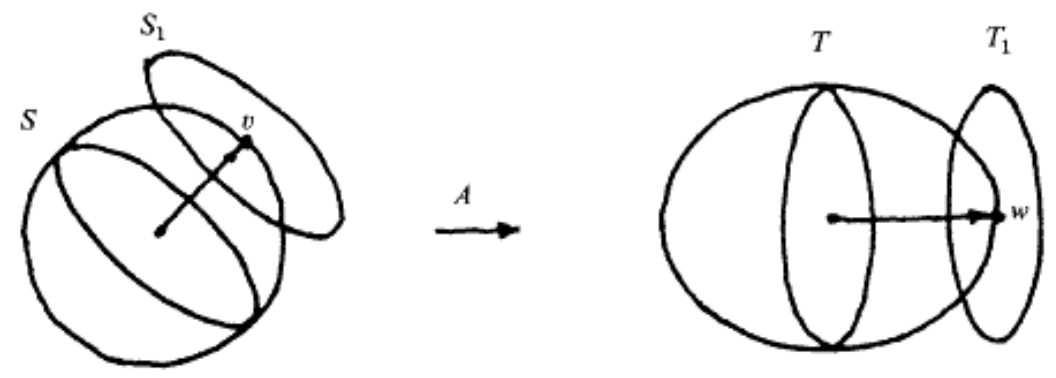
\includegraphics[width=13cm]{svd-geo-proof}
  \caption{Geometrical proof of SVD Theorem: Transformation $A$ preserves the
    relation $S \perp \vec{v}$}
  \label{fig:svdgeop}
\end{figure}
\hfill

\begin{proof}
The geometric proof goes like this: \\

\begin{enumerate}
\item The hyperplane $S_1$ touches the unit sphere only at point
  \vec{v}. It is a geometrical result that such hyperplane is unique
  and that $S_1 \perp \vec{v}$. \\

\item By definition, the hyperplane $T_1$ is the image of $S_1$ under
  $A$; also, the whole unit sphere is mapped by $A$ into an ellipsoid. Since
  $A$ is a bijective function, then $T_1$ must touch the ellipsoid only in
  point \vec{w} (just like $S_1$ touches the unit sphere only at point
  \vec{v}). Actually, $T_1$ must be the only hyperplane with such
  property (otherwise, we could apply \inv{A} to that other hyperplane,
  and it would produce a different hyperplane that also touches
  \vec{v} in the unit sphere; contradicting previous point about the
  uniqueness of $S_1$). \\

\item Now take another sphere, big enough to cover the deformed image of
  the unit sphere under $A$ (the ellipsoid). Start to shrink
  such sphere until it touches the ellipsoid for the first time; per
  definition, \vec{w} must be part of those points of first
  contact. \\

\item Now consider the hyperplane $T_2$ that touches this shrunk sphere,
  precisely at \vec{w}. Using the same geometrical theorem of first
  argument about $S_1$, we can tell such hyperplane is unique and is
  orthogonal to \vec{w}. \\

\item Since this adjusted sphere covers entirely the ellipsoid (per
  definition of \vec{w}), then $T_2$ also touches the ellipsoid at
  point \vec{w}. But we argued that $T_1$ was the only hyperplane
  touching the ellipsoid at \vec{w} $\implies$ $T_1 = T_2 \ds{\land} T_1
  \perp \vec{w}$. \\

\item Both hyperplanes $S$ and $S_1$ are orthogonal to \vec{v}; by
  geometrical arguments they must be parallel then. \\

\item Linear transformations, in particular $A$, preserve parallelism;
  since, $S \parallel S_1$ $\implies$ their respective images under $A$
  must be parallel as well. \\

\item The image of $S_1$ under $A$ is $T_1$, then, whatever becomes
  the image of $S$ under $A$; it must be parallel to $T_1$. Let us
  call this image $T$. \\

\item $\therefore$ $T \parallel T_1 \ds{\land} T_1 \perp \vec{w}$
  $\implies$ $T \perp \vec{w}$.  
\end{enumerate}
\end{proof}
\hfill

The key choice in the proof was \vec{w}, as being the biggest axis of
the ellipsoid makes it coincide with the sphere of radius
$\norm{w}_2$; and that in turns allows us to transfer the properties
of the hyperplane that touches the sphere at \vec{w} to the one that
touches the ellipsoid at same point (as they become same hyperplane
indeed). It is no coincidence then, that the spectral norm $\norm{A}_2$
is actually defined as $\norm{\vec{w}}_2$; that is, is defined
as the maximum expansion $\norm{A\vec{x}}_2$ that transformation $A$ causes
on the vectors belonging to the unit sphere. This norm actually, is
used in the algebraic proof of Golub in \cite{golub13}, of the SVD
Theorem. \\ 

The last question the reader may have now is: where was the
compactness property used? It may not be explicitly stated, but it
lies behind the definition of \vec{w}: $\norm{\vec{w}}_2 =
\max\left\{\norm{\vec{x}}_2 \suchthat \norm{\inv{A}\vec{x}}_2 = 1
\right\}$. The reason why \vec{w} exists 
on the first place, is because the ellipsoid is a compact set (it
inherits that property from its pre-image, the unit sphere, thanks to
the continuity of function $A$\footnote{Though we did not find the
  name for such theorem, it must exists and state that continuous
  functions preserve compactness.}). Since the norm function $\norm{.}_2$
is also continuous, then by a generalization of the Extreme Value
Theorem from Calculus, it must reach its maximum on a point of the
ellipsoid (we named that particular point as \vec{w} in the proof). \\



